\documentclass[tikz,border=10pt]{standalone}
% Load calc library for the $(Q)+(...)$ right-angle mark coordinates
\usetikzlibrary{calc}
% Scale s = 0.008538 units/px, origin shifted to B for readability (y flipped)
\begin{document}
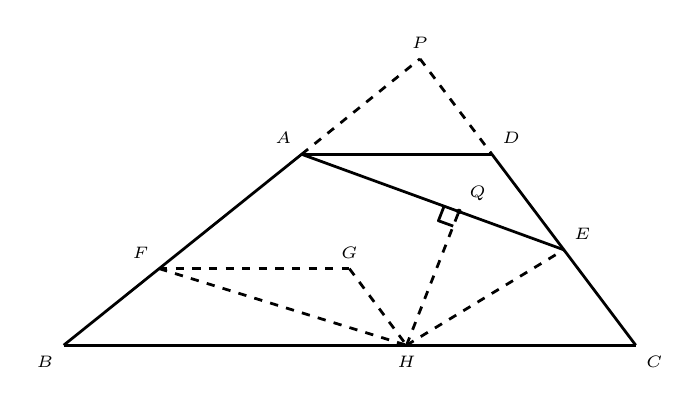
\begin{tikzpicture}[line width=1.0pt, line join=round]
  % Named points (converted from pixel coordinates)
  \coordinate (B) at (0,0);
  \coordinate (H) at (4.354,0);
  \coordinate (C) at (7.265,0);
  \coordinate (A) at (3.022,2.425);
  \coordinate (F) at (1.212,0.973);
  \coordinate (E) at (6.352,1.212);
  \coordinate (Q) at (5.020,1.699);
  \coordinate (D) at (5.439,2.425);
  \coordinate (G) at (3.628,0.973);
  \coordinate (P) at (4.525,3.637);

  % Solid segments
  \draw (B) -- (C);
  \draw (B) -- (A);
  \draw (A) -- (D);
  \draw (D) -- (C);
  \draw (A) -- (E);

  % Dashed segments
  \draw[dashed] (A) -- (P);
  \draw[dashed] (P) -- (D);
  \draw[dashed] (F) -- (G);
  \draw[dashed] (G) -- (H);
  \draw[dashed] (F) -- (H);
  \draw[dashed] (H) -- (Q);
  \draw[dashed] (H) -- (E);

  % Right-angle mark at Q (between QA and QH), side 0.2
  \draw ($(Q)+(-0.188,0.068)$) -- ($(Q)+(-0.261,-0.118)$) -- ($(Q)+(-0.073,-0.186)$);

  % Vertex dots/labels
  \fill (Q) circle (1pt);
  \node[above left, font=\fontsize{6}{7.2}\selectfont] at (A) {$A$};
  \node[above right, font=\fontsize{6}{7.2}\selectfont] at (D) {$D$};
  \node[above right, font=\fontsize{6}{7.2}\selectfont] at (E) {$E$};
  \node[above left, font=\fontsize{6}{7.2}\selectfont] at (F) {$F$};
  \node[above, font=\fontsize{6}{7.2}\selectfont] at (G) {$G$};
  \node[below, font=\fontsize{6}{7.2}\selectfont] at (H) {$H$};
  \node[below left, font=\fontsize{6}{7.2}\selectfont] at (B) {$B$};
  \node[below right, font=\fontsize{6}{7.2}\selectfont] at (C) {$C$};
  \node[above right, font=\fontsize{6}{7.2}\selectfont] at (Q) {$Q$};
  \node[above, font=\fontsize{6}{7.2}\selectfont] at (P) {$P$};
\end{tikzpicture}
\end{document}